%% HEAD from knitr template
%% /Users/abarbour/Library/textemplates
%% Thu Feb  7 18:24:57 PST 2013
\documentclass[10pt]{article}\usepackage{graphicx, color}
%% maxwidth is the original width if it is less than linewidth
%% otherwise use linewidth (to make sure the graphics do not exceed the margin)
\makeatletter
\def\maxwidth{ %
  \ifdim\Gin@nat@width>\linewidth
    \linewidth
  \else
    \Gin@nat@width
  \fi
}
\makeatother

\definecolor{fgcolor}{rgb}{0.2, 0.2, 0.2}
\newcommand{\hlnumber}[1]{\textcolor[rgb]{0,0,0}{#1}}%
\newcommand{\hlfunctioncall}[1]{\textcolor[rgb]{0.501960784313725,0,0.329411764705882}{\textbf{#1}}}%
\newcommand{\hlstring}[1]{\textcolor[rgb]{0.6,0.6,1}{#1}}%
\newcommand{\hlkeyword}[1]{\textcolor[rgb]{0,0,0}{\textbf{#1}}}%
\newcommand{\hlargument}[1]{\textcolor[rgb]{0.690196078431373,0.250980392156863,0.0196078431372549}{#1}}%
\newcommand{\hlcomment}[1]{\textcolor[rgb]{0.180392156862745,0.6,0.341176470588235}{#1}}%
\newcommand{\hlroxygencomment}[1]{\textcolor[rgb]{0.43921568627451,0.47843137254902,0.701960784313725}{#1}}%
\newcommand{\hlformalargs}[1]{\textcolor[rgb]{0.690196078431373,0.250980392156863,0.0196078431372549}{#1}}%
\newcommand{\hleqformalargs}[1]{\textcolor[rgb]{0.690196078431373,0.250980392156863,0.0196078431372549}{#1}}%
\newcommand{\hlassignement}[1]{\textcolor[rgb]{0,0,0}{\textbf{#1}}}%
\newcommand{\hlpackage}[1]{\textcolor[rgb]{0.588235294117647,0.709803921568627,0.145098039215686}{#1}}%
\newcommand{\hlslot}[1]{\textit{#1}}%
\newcommand{\hlsymbol}[1]{\textcolor[rgb]{0,0,0}{#1}}%
\newcommand{\hlprompt}[1]{\textcolor[rgb]{0.2,0.2,0.2}{#1}}%

\usepackage{framed}
\makeatletter
\newenvironment{kframe}{%
 \def\at@end@of@kframe{}%
 \ifinner\ifhmode%
  \def\at@end@of@kframe{\end{minipage}}%
  \begin{minipage}{\columnwidth}%
 \fi\fi%
 \def\FrameCommand##1{\hskip\@totalleftmargin \hskip-\fboxsep
 \colorbox{shadecolor}{##1}\hskip-\fboxsep
     % There is no \\@totalrightmargin, so:
     \hskip-\linewidth \hskip-\@totalleftmargin \hskip\columnwidth}%
 \MakeFramed {\advance\hsize-\width
   \@totalleftmargin\z@ \linewidth\hsize
   \@setminipage}}%
 {\par\unskip\endMakeFramed%
 \at@end@of@kframe}
\makeatother

\definecolor{shadecolor}{rgb}{.97, .97, .97}
\definecolor{messagecolor}{rgb}{0, 0, 0}
\definecolor{warningcolor}{rgb}{1, 0, 1}
\definecolor{errorcolor}{rgb}{1, 0, 0}
\newenvironment{knitrout}{}{} % an empty environment to be redefined in TeX

\usepackage{alltt}
%%
%% !Rnw weave = knitr
%% sweave fig help:
%% http://users.stat.umn.edu/~geyer/Sweave/foo.pdf
%%
% \VignetteIndexEntry{ResponseModels}
% \VignetteEngine{knitr}
%
\usepackage{amsmath}
\usepackage{amssymb}
\usepackage[font=sf, labelfont={sf,bf}, margin=2cm]{caption}
\usepackage[T1]{fontenc}
\usepackage[utf8]{inputenc}
\usepackage{fancyvrb}
\usepackage{float}
\usepackage{geometry}
\geometry{verbose,tmargin=3cm,bmargin=5cm,lmargin=2.5cm,rmargin=2.5cm}
\usepackage{graphicx}
\usepackage{grffile}
\usepackage[pdfborder={0 0 0}]{hyperref}
\usepackage[utf8]{inputenc}
\usepackage{natbib}
\usepackage{makeidx}
\makeindex % comment to have no index
\usepackage{upquote}
\usepackage{url}
%
\author{Andrew J. Barbour}
\title{Demonstration of Well Response Functions}
\IfFileExists{upquote.sty}{\usepackage{upquote}}{}
\begin{document}
\maketitle
%\tableofcontents
%% BODY from knitr template
%\newcommand{\newcomm}[1]{#1}
%\renewcommand{\newcomm}[1]{#1}
%
\newcommand{\SC}[1]{\textsc{#1}}
\newcommand{\Rcmd}[1]{\texttt{#1}}
\newcommand{\bidxa}[1]{\index{#1}{\textbf{#1}}} 
\newcommand{\bidxb}[2]{\index{#2}{\textbf{#1}}} 
\newcommand{\idxa}[1]{\index{#1}{#1}} 
\newcommand{\idxb}[2]{\index{#2}{#1}} 
%
\begin{abstract}
abstract text
\end{abstract}
%
\section{Sealed well response}
\subsection{Strain: Kitagawa (2011)}
%
\citet{kitagawa2011}

\section{Open well response}
\subsection{Strain: Rojstaczer (1988)}
%
\citet{rojstaczer1988, rojstaczer1988b}

Load the packages
\begin{knitrout}
\definecolor{shadecolor}{rgb}{0.969, 0.969, 0.969}\color{fgcolor}\begin{kframe}
\begin{alltt}
\hlfunctioncall{library}(signal, warn.conflicts = FALSE)
\end{alltt}


{\ttfamily\noindent\itshape\color{messagecolor}{\#\# Loading required package: MASS}}\begin{alltt}
\hlfunctioncall{library}(kitagawa, warn.conflicts = FALSE)
\end{alltt}


{\ttfamily\noindent\itshape\color{messagecolor}{\#\# Loading required package: kelvin}}

{\ttfamily\noindent\itshape\color{messagecolor}{\#\# Loading required package: Bessel}}

{\ttfamily\noindent\itshape\color{messagecolor}{\#\# Loading required package: Rmpfr}}

{\ttfamily\noindent\itshape\color{messagecolor}{\#\# Loading required package: gmp}}

{\ttfamily\noindent\itshape\color{messagecolor}{\#\# \\\#\# Attaching package: 'gmp'}}

{\ttfamily\noindent\itshape\color{messagecolor}{\#\# The following object is masked from 'package:base':\\\#\# \\\#\#\ \ \ \  \%*\%, apply, crossprod, matrix, tcrossprod}}\begin{verbatim}
## Loading C code of R package 'Rmpfr': GMP using 64 bits per limb
\end{verbatim}


{\ttfamily\noindent\itshape\color{messagecolor}{\#\# \\\#\# Attaching package: 'Rmpfr'}}

{\ttfamily\noindent\itshape\color{messagecolor}{\#\# The following object is masked from 'package:stats':\\\#\# \\\#\#\ \ \ \  pnorm, print.integrate}}

{\ttfamily\noindent\itshape\color{messagecolor}{\#\# The following object is masked from 'package:base':\\\#\# \\\#\#\ \ \ \  cbind, pmax, pmin, rbind}}

{\ttfamily\noindent\itshape\color{messagecolor}{\#\# Loaded kelvin (1.2.2) -- Solutions to the Kelvin differential equation.}}

{\ttfamily\noindent\itshape\color{messagecolor}{\#\# Loaded kitagawa (2.0.2) -- Spectral response of water wells}}\end{kframe}
\end{knitrout}

%#library(kook) # locally only
%# Note Rmpfr has erf and erfc functions... 
%
\begin{knitrout}
\definecolor{shadecolor}{rgb}{0.969, 0.969, 0.969}\color{fgcolor}\begin{kframe}
\begin{alltt}
omega <- 10^\hlfunctioncall{seq}(-3, 2, by = 0.1)
z <- 1
Trans <- 1
Stor <- 1
Diffus <- Trans/Stor
\hlcomment{# nondim freq}
Q <- 10^\hlfunctioncall{seq}(-3, 2, by = 0.1)  \hlcomment{# == z**2 omega / 2 D}
omega <- Q * 2 * Diffus/z^2
wrsp <- \hlfunctioncall{open_well_response}(omega, T. = Trans, S. = Stor, z. = z, model = \hlstring{"rojstaczer"})
crsp <- wrsp[, 2]
\hlcomment{#}
lQ <- \hlfunctioncall{log10}(Q)
\hlcomment{# Amplitude}
As <- 0.05  \hlcomment{# cm/nE}
Gain <- \hlfunctioncall{Mod}(crsp)
\hlcomment{# Phase}
Phs <- \hlfunctioncall{Arg}(crsp)  \hlcomment{# will wrap to -pi/pi}
uPhs <- signal::\hlfunctioncall{unwrap}(Phs, tol = pi/30)
\end{alltt}
\end{kframe}
\end{knitrout}


\begin{figure}[htb!]
\begin{center}
\begin{knitrout}
\definecolor{shadecolor}{rgb}{0.969, 0.969, 0.969}\color{fgcolor}
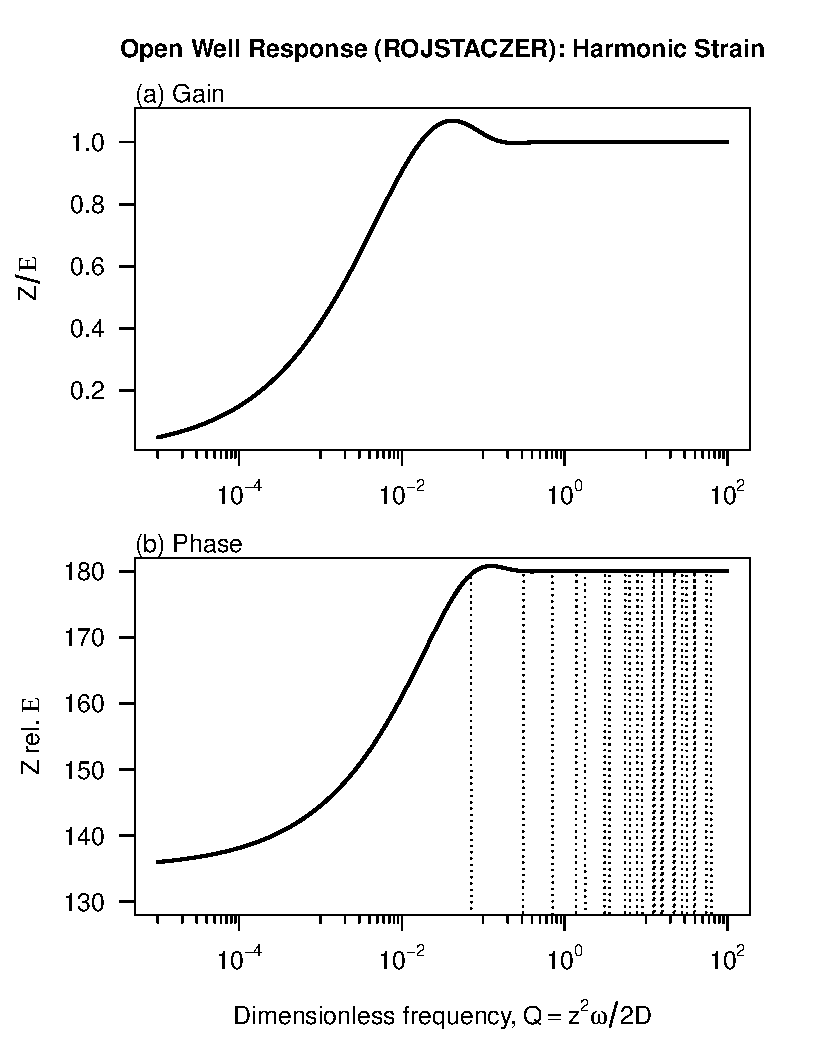
\includegraphics[width=\maxwidth]{figure/ROJRESPFIG} 

\end{knitrout}

\caption{The response of an open well to harmonic areal strains, using
the model of \citet{rojstaczer1988}.}
\label{fig:tmp}
\end{center}
\end{figure}

%% TAIL from knitr template
\bibliographystyle{apalike}
\bibliography{REFS}

\printindex

\end{document}
